A certain set of calibration constants is valid over a period of time called
\gls{iov}. The cell noise can vary due to a change in the calibration, the
digital noise or the channel status in a particular run. This change must be
consistent and checked.

The different TileCal subsystems (laser, CIS, etc.) all use a common software
framework, \gls{tucs}, to perform validity checks on a number of different
studies. To test the stability over time of the updated noise constants, a set
of python scripts was developed to expand the TUCS functionality. These scripts
allow to visually display the relative change of the cell noise and digital
noise constants, the channel status and the ratio between the cell noise and a
variable called RMS$_\text{eff}$ and defined as:
\begin{equation}
  \label{eq:73}
  \text{RMS}_{\text{eff}} = \sqrt{(1 - R) \sigma_1^2 + R \sigma_2^2}
\end{equation}
where $\sigma_1$, $\sigma_2$ and R are the free parameter in the double Gaussian
model (see Section~\ref{sec:cell-noise}).  The ratio $\sigma$ /
RMS$_\text{eff}$, where $\sigma$ is the cell noise, can be used to test the
goodness of the double Gaussian model: if $\sigma$ / RMS$_\text{eff}$ equals
one, the double Gaussian well models the noise, if it is larger, it means that
there is noise that is not well described by it.

Figure~\ref{fig:jumps} shows the time evolution plot for two representative
TileCal cells. In Figure~\ref{fig:no_jumps} it can be seen that cell number 2 in
the BC layer (BC2) of the 41st module in the C side of LB (LBC 41) is stable
over several pedestal runs. In Figure~\ref{fig:with_jumps} on the other hand, it
is possible to see a variation in the cell noise and, accordingly, of the
$\sigma$ / RMS$_{\text{eff}}$ without a compatible variation in the calibration,
in the digital noise constants or in the channel status. The term \emph{jump}
will be used in the following to indicate a variation in the cell noise not
compatible with a change in the other quantities.

\begin{figure}[!h]
  \centering
  \begin{subfigure}[t]{.48\linewidth}
    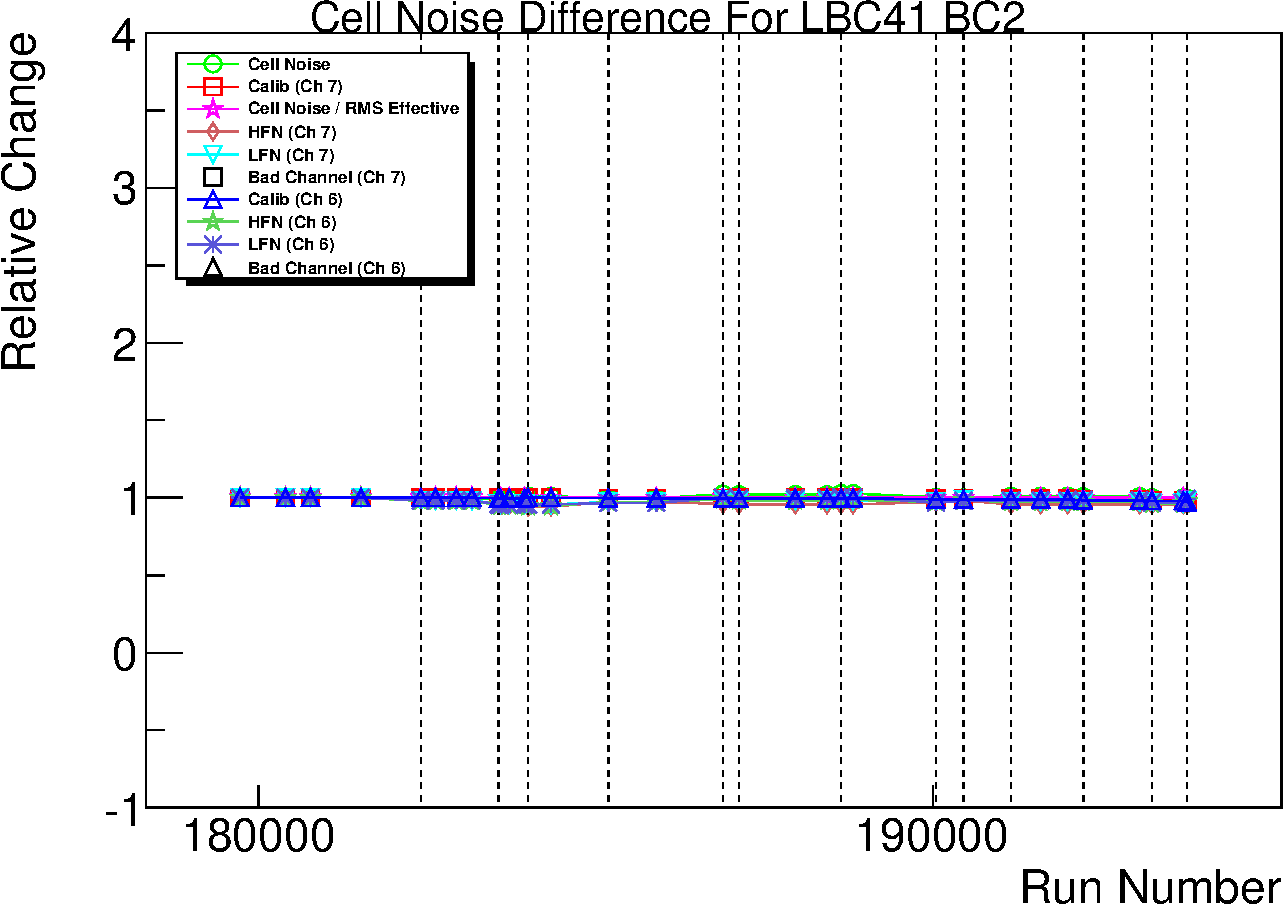
\includegraphics[width=\linewidth]{no_jumps}
    \caption{}
    \label{fig:no_jumps}
  \end{subfigure}
  \begin{subfigure}[t]{.48\linewidth}
    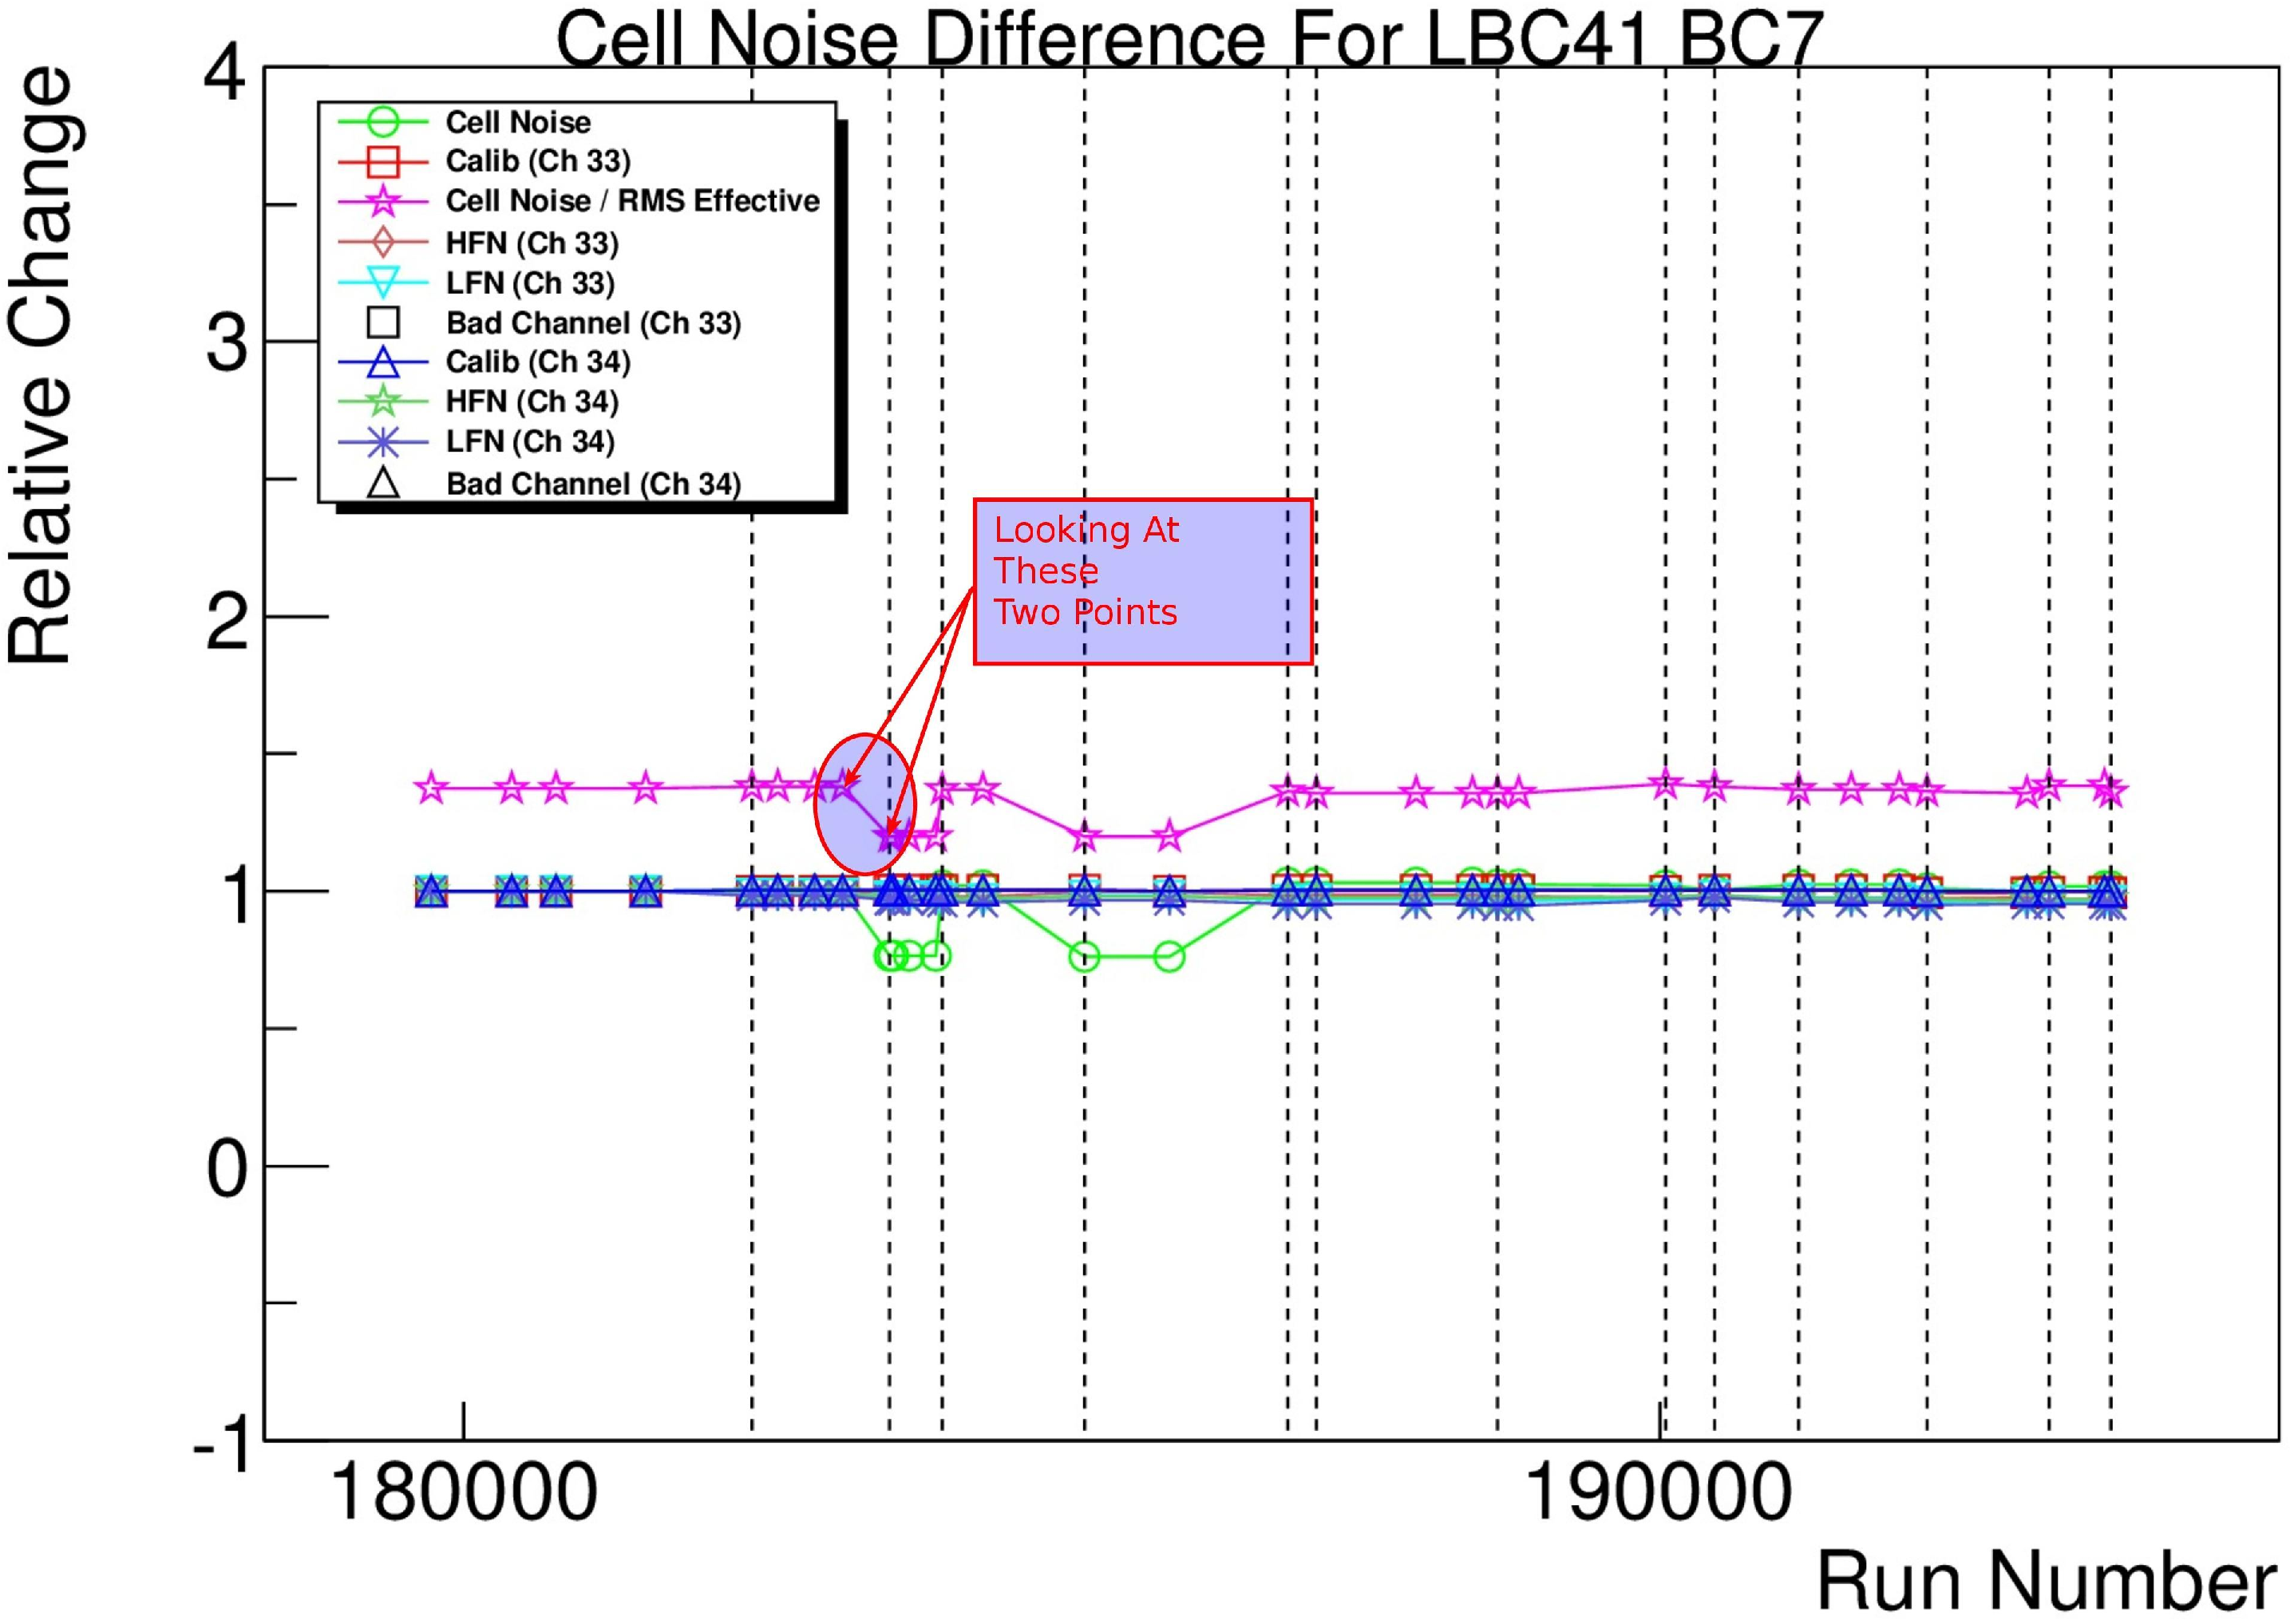
\includegraphics[width=\linewidth]{with_jumps}
    \caption{}
    \label{fig:with_jumps}
  \end{subfigure}
  \caption{Time evolution plots for two different representative cells in the
    calorimeter. The plot shows the change relative to the first run considered
    of several quantities for different IOVs (vertical dashed lines).}
  \label{fig:jumps}
\end{figure}

This problem was investigated by writing a software to manually fit the pulse
shape and calculate the noise constants focusing on two specific IOVs,
$[183110, 183382[$ and $[183382, 183515[$. Some calorimeter cells without jump
were used to validate the noise constants calculated with the fit and those
stored in the COOL database. Figure~\ref{fig:no_jump_fit} shows the control cell
energy distribution with the double Gaussian fit superimposed for two runs where
the jump was present in other cells. The results for the ratio of the amplitude
of the double Gaussian model (R), the RMS$_{\text{eff}}$ and the $\sigma$ /
RMS$_{\text{eff}}$ obtained with the fit are:
\begin{equation}
  \begin{cases}
    R : 0.0003 \\
    \text{RMS}_{\text{eff}}: 20.12 \\
    \sigma / \text{RMS}_{\text{eff}}: 0.998
  \end{cases}
  \to
  \begin{cases}
    R : 0.0002 \\
    \text{RMS}_{\text{eff}} : 20.07 \\
    \sigma / \text{RMS}_{\text{eff}}: 0.995.
  \end{cases}
  \label{eq:74}
\end{equation}
They are in good agreement with the values stored in the COOL database and
reported in Table~\ref{tab:no_jump_fit}.

\begin{figure}[!h]
  \centering
  \begin{subfigure}[t]{.48\linewidth}
    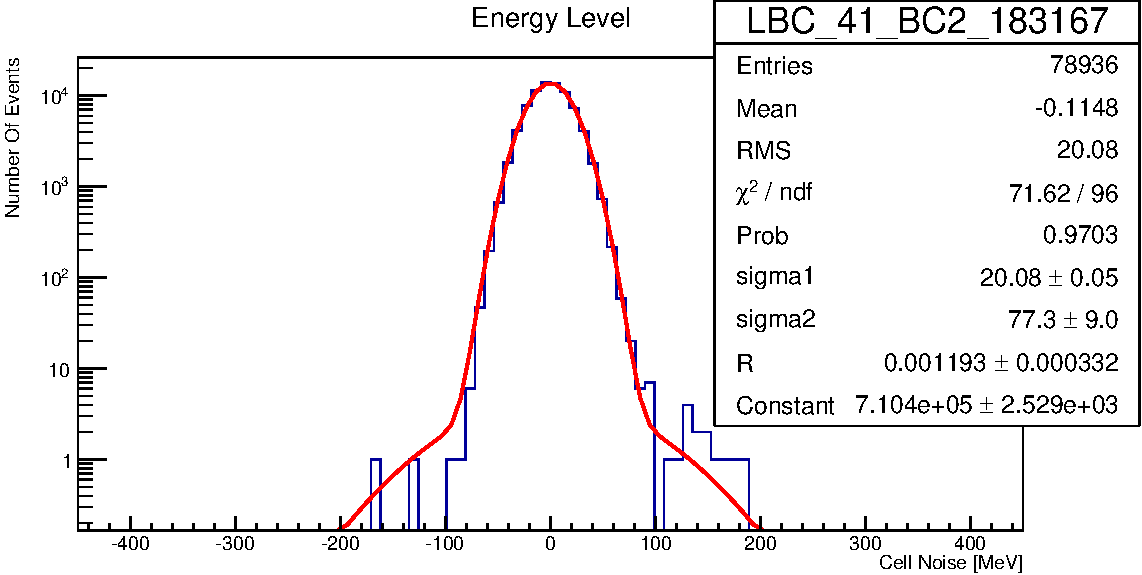
\includegraphics[width=\linewidth]{no_jump_fit_before}
    \caption{Fit before jump.}
    \label{fig:no_jump_fit_before}
  \end{subfigure}
  \begin{subfigure}[t]{.48\linewidth}
    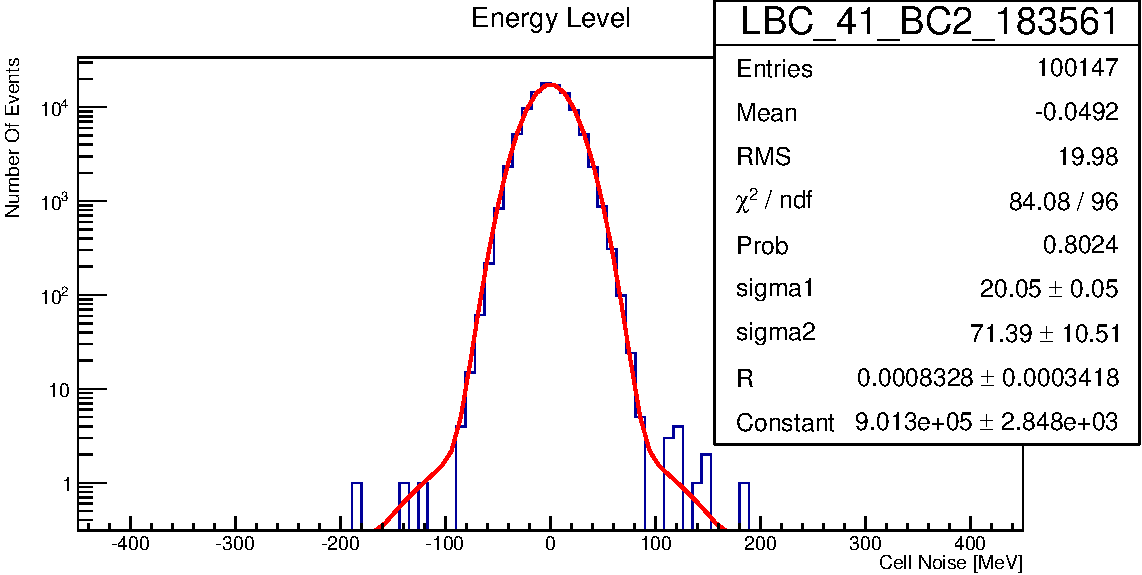
\includegraphics[width=\linewidth]{no_jump_fit_after}
    \caption{Fit after jump.}
    \label{fig:no_jump_fit_after}
  \end{subfigure}
  \caption{Fit of the reconstructed pulse shape on a control cell with no
    variation (jump) in the cell noise.}
  \label{fig:no_jump_fit}
\end{figure}

\begin{table}[!h]
  \centering
  \begin{tabular}{r c}
    \multicolumn{2}{c}{LBC41 BC2 Values From Database} \\
    \hline \hline
    \multicolumn{2}{c}{Before Jump} \\
    \hline \hline
    $\sigma$: & 20.08 \\
    $\sigma_1$: & 19.97 \\
    $\sigma_2$: & 80.59 \\
    R\@: & 0.00026 \\
    RMS$_\text{eff}$: & 20.01 \\
    $\sigma$ / RMS$_\text{eff}$: & 1.0035 \\
    \hline \hline
  \end{tabular} \quad
  \begin{tabular}{r c}
    \multicolumn{2}{c}{LBC41 BC2 Values From Database} \\
    \hline \hline
    \multicolumn{2}{c}{After Jump} \\
    \hline \hline
    $\sigma$: & 19.98 \\
    $\sigma_1$: & 19.94 \\
    $\sigma_2$: & 71.41 \\
    R\@: & 0.00023 \\
    RMS$_\text{eff}$: & 19.97 \\
    $\sigma$ / RMS$_\text{eff}$: & 1.0006 \\
    \hline \hline
  \end{tabular}
  \caption{The table reports the cell noise constants stored in the COOL
    database for two different run numbers corresponding to before and after the
  jump for a cell where there is no variation in the cell noise.}
\label{tab:no_jump_fit}
\end{table}

Figure~\ref{fig:jump_fit} shows the energy distribution with the double Gaussian
fit superimposed on the seventh cell of the BC layer (BC7) on the C side of the
LB partition of the 41st module (LBC 41). The cell had the jump under
investigation (see Figure~\ref{fig:jumps}) and this is reflected in the fit results:
\begin{equation}
  \label{eq:75}
  \begin{cases}
    R : 0.042 \\
    \text{RMS}_{\text{eff}}: 29.59 \\
    \sigma / \text{RMS}_{\text{eff}}: 1.37
  \end{cases}
  \to
  \begin{cases}
    R : 0.014 \\
    \text{RMS}_\text{{eff}} : 26.67 \\
    \sigma / \text{RMS}_{\text{eff}}: 1.2.
  \end{cases}
\end{equation}
Also in this case, the noise constants from the fit, are in agreement with those
stored in the COOL database and reported in  Table~\ref{tab:jump_fit}. Moreover,
the $\chi^2$ of the distribution and the ration $\sigma$ / RMS$_{\text{eff}}$
greater than one, imply that the double Gaussian model is not a good model in
this case.

\begin{figure}[!h]
  \centering
  \begin{subfigure}[t]{.48\linewidth}
    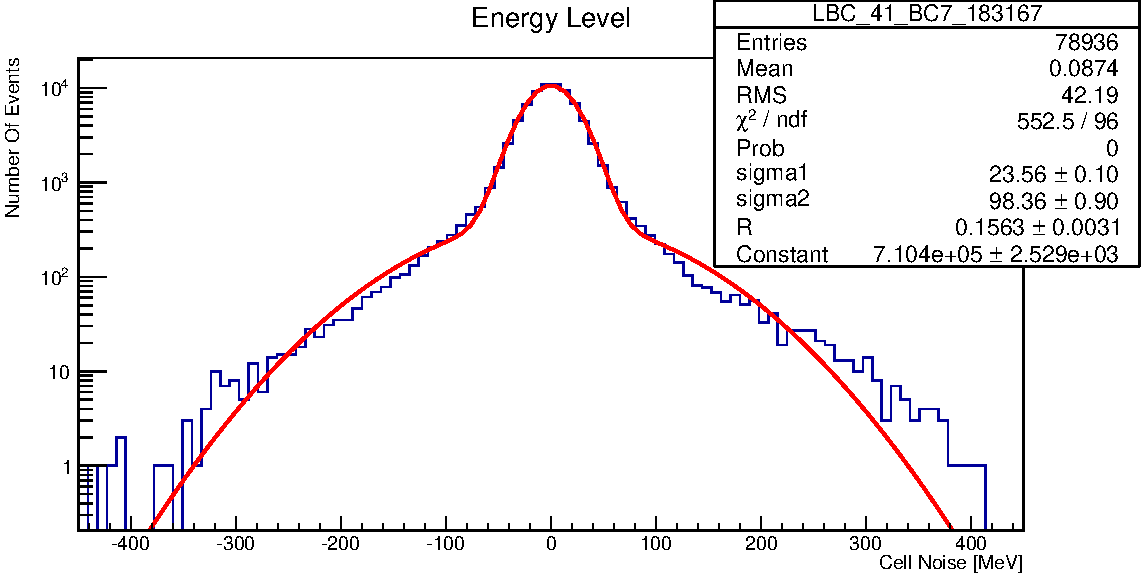
\includegraphics[width=\linewidth]{jump_fit_before}
    \caption{Before jump.}
    \label{fig:jump_fit_before}
  \end{subfigure}
  \begin{subfigure}[t]{.48\linewidth}
    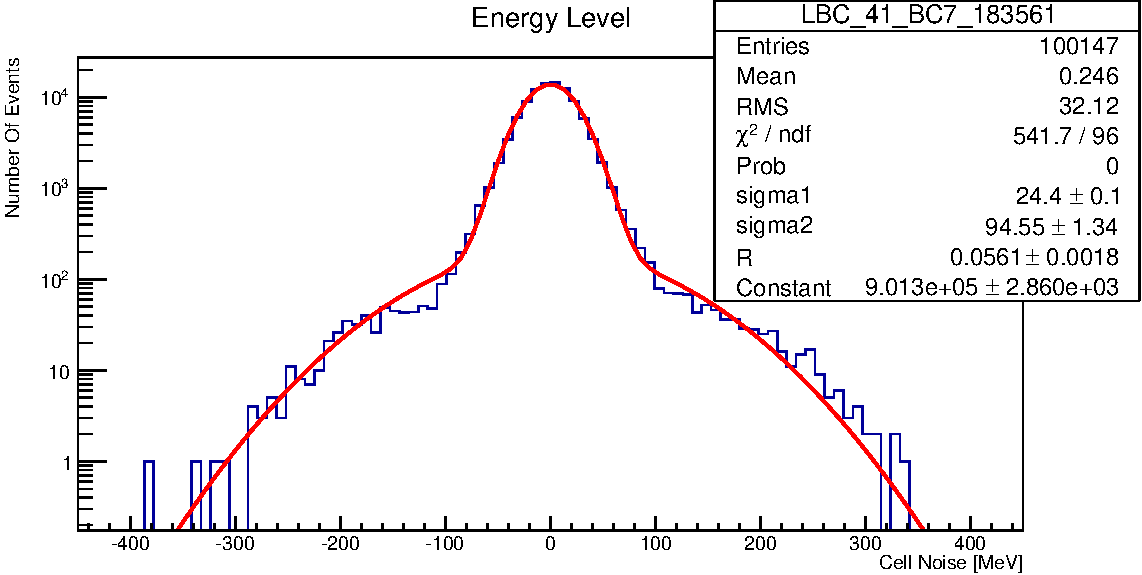
\includegraphics[width=\linewidth]{jump_fit_after}
    \caption{After jump.}
    \label{fig:jump_fit_after}
  \end{subfigure}
  \caption{Fit of the reconstructed pulse shape on a cell with variation (jump)
    in the cell noise non compatible with a change in the calibration, digital
    noise or channel status.}
  \label{fig:jump_fit}
\end{figure}

\begin{table}[!h]
  \centering
  \begin{tabular}{r c}
    \multicolumn{2}{c}{LBC41 BC7 Values From Database} \\
    \hline \hline
    \multicolumn{2}{c}{Before Jump} \\
    \hline \hline
    $\sigma$: & 42.19 \\
    $\sigma_1$: & 24.26 \\
    $\sigma_2$: & 99.16 \\
    R\@: & 0.037 \\
    RMS$_{\text{eff}}$: & 30.56 \\
    $\sigma$ / RMS$_{\text{eff}}$: & 1.38 \\
    \hline \hline
  \end{tabular} \quad
  \begin{tabular}{r c}
    \multicolumn{2}{c}{LBC41 BC7 Values From Database} \\
    \hline \hline
    \multicolumn{2}{c}{After Jump} \\
    \hline \hline
    $\sigma$: & 32.12 \\
    $\sigma_1$: & 24.42 \\
    $\sigma_2$: & 94.56 \\
    R\@: & 0.014 \\
    RMS$_{\text{eff}}$: & 26.79 \\
    $\sigma$ / RMS$_{\text{eff}}$: & 1.20 \\
    \hline \hline
  \end{tabular}
  \caption{The table reports the cell noise constants stored in the COOL
    database for two different run numbers corresponding to before and after the
  jump for a cell where there is a variation in the cell noise was spotted.}
  \label{tab:jump_fit}
\end{table}

After consultation with experts~\cite{PrivateConv}, it was suggested that this
behavior could be caused by the \gls{tnf}. Many electronic devices are involved
in the signal reconstruction, the noise of these can be altered in a coherent
way (by electromagnetic field emission for instance) and thus altering the jet
and missing transverse energy reconstruction. This alteration is called
\emph{coherent noise} and what the TNF does is to subtract it from the channels
connected to the same motherboard (see Section~\ref{sec:sign-reconstr}) on an
event-by-event basis. The cell noise war recalculated without without noise
filter and the corresponding distribution re-fitted obtaining:
\begin{equation}
  \label{eq:76}
  \begin{cases}
    R : 0.0750867 \\
    \text{RMS}_\text{eff} : 47.49 \\
    \sigma / \text{RMS}_\text{eff}: 1.49
  \end{cases}
  \to
  \begin{cases}
    R : 0.075  \\
    \text{RMS}_\text{eff}: 48.91 \\
    \sigma / \text{RMS}_\text{eff}: 1.44.
  \end{cases}
\end{equation}
Comparing Equation~\ref{eq:76} with Equation~\ref{eq:75} it is possible to see
that without TNF, there is no jump.
%%% Local Variables:
%%% mode: latex
%%% TeX-master: "../search_for_DM_LED_with_ATLAS"
%%% End:
